\documentclass[]{article}

\usepackage{graphicx} %for å inkludere grafikk
\usepackage{verbatim} %for å inkludere filer med tegn LaTeX ikke liker
\usepackage{tabularx}
\usepackage{booktabs}
\usepackage{amsmath}
\usepackage{float}
\usepackage{color}
\usepackage{listings}
\usepackage{physics}
\usepackage{hyperref}
\usepackage{subfig}
\usepackage{mhchem}
\usepackage{natbib}
%opening
\title{}
\author{}

\begin{document}
	
\title{Fission: a TALYS report}
\author{Dorthea Gjestvang }
\date{December 2017}

\maketitle

\begin{abstract}

\end{abstract}

\section{Introduction}

\section{Theory}
\subsection{Fission barrier}
When observing the average binding energy per nucleon, as seen in Figure \ref{fig:binding_energy_per_nucleon}, one can see that for $A \approx 60$ the binding energy per A peaks, and then starts to decrease for increasing A. For nuclei situated to the right of this peak, it is thus possible to release energy by splitting in two lighter fragments, that is to fission. However, when studying the chart of nuclei , one will observe that only a handfull of nuclei have spontaneous fission as their main decay mode, and they are generally heavy elements far from the valley of stability. This  is due to the so-called fission barrier. 
\par
\vspace{3mm}

\begin{figure}
	\centering
	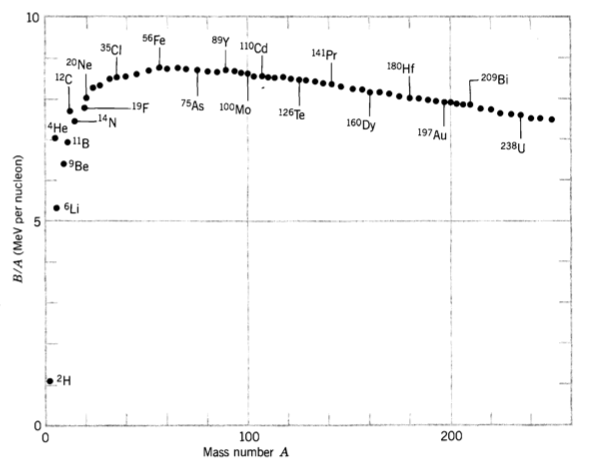
\includegraphics[scale=0.6]{binding_energy_per_nucleon.png}
	\caption{Average binding energy per nucleon. Figure from K.S. Krane p.67 \cite{Krane1988}}
	\label{fig:binding_energy_per_nucleon}
\end{figure}


 \noindent In the liquid model, the fission barrier is described as a smooth, parabolic barrier, and is shown in Figure \ref{fig:smooth_fission_barrier}. It describes the energy needed to separate the two fission fragments as a function of separation distance. The fission barrier is due to both the nuclear force and the Coloumb force. A picture on why there is a fission barrier, is that in order for the two would-be fission fragments to separate, they have to get out of the potential well that is the nuclear force, and then pass the Coloumb barrier surrounding the nucleus. Thus energy must be applied for the fragments to be able to separate. This energy needed is often referred to as the activation energy, and is shown in Figure \ref{fig:smooth_fission_barrier} as the difference in energy between the ground state of the nucleus, and the maximum of the fission barrier potential. 
 
 \par
 \vspace{3mm}
 
 \begin{figure}
 	\centering
 	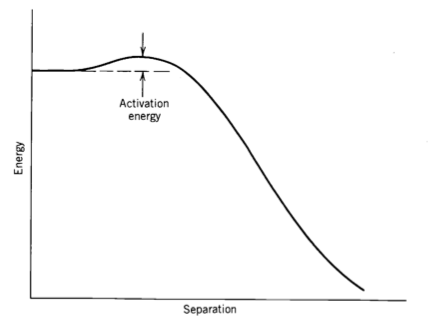
\includegraphics[scale=0.7]{smooth_fission_barrier.png}
 	\caption{The smooth fission barrier, illustrating the activation energy. Figure from K.S. Krane p.481 \cite{Krane1988}}
 	\label{fig:smooth_fission_barrier}
 \end{figure}

\noindent The energy released in fission is about the same as the activation energy needed to overcome the fission barrier. Those nuceli that have an energy release though fission that allows them to overcome most of the fission barrier, have a highter probability of tunnelling through the barrier \cite{Krane1988} (p.481). This is a known effect from quantum physics: the thinner the potential barrier, the larger the probability of tunnelling. These nuclei that see a thin potential barrier are thus called the spontaneously fissioning nuclei. However, most of the nuceli are not able to overcome much fission barrier by themselves, and thus they see a thick potential, and the probability of tunnelling is vanishing. They are therefore not unstable to spontaneous fission. This explains why the number of spontaneously fissioning nuclei are so few, even though it is energetically possible for plenty of the heavier nuclei to fission.

\par
\vspace{3mm}

\noindent This far I´ve only described the fission barrier using the liquid drop model. However, the liquid drop model is not a complete description of the nuclei, and shell effects have a impact when studying the probability to fission. When including the effects of the single particle shell structure, the fission barrier is changed to a barrier with two humps, called the double-humped fission barrier \cite{Krane1988} (p.495). The double-humped fission barrier is shown in Figure \ref{fig:double_humped_fission_barrier}. Nucei with energies well below the fission barrier , but above the well in the fission potential, thus sees two thinner barriers, compared to one thick barrier that the nuclei sees if it has energies below this well. They can tunnel through the first barrier, and then exist in an isomer state in the well, before either tunnelling through the second ponential hump, or gamma-decay back to the ground state.  The tunnelling of two thin barriers is more probable than tunnelling through one thick barrier, so the double-humped fission barrier makes more nuclei unstable to spontaneous fission. The existence of the double-humped fission barrier was confirmed when fission isomers were discovered, which are isotopes highly unstable to spontaneous fission \cite{Krane1988} (p.495). 

  \begin{figure}
 	\centering
 	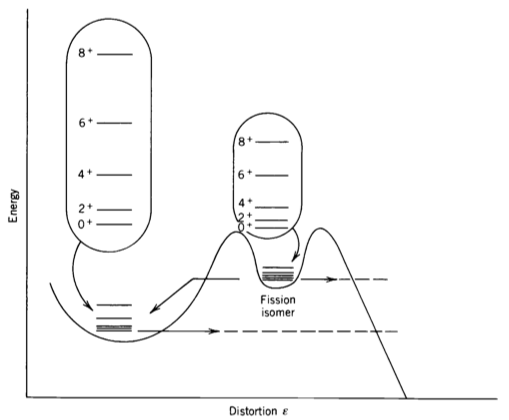
\includegraphics[scale=0.7]{double_humped_fission_barrier.png}
 	\caption{The double humped fission barrier Figure from K.S. Krane p.496 \cite{Krane1988}}
 	\label{fig:smooth_fission_barrier}
 \end{figure}

\noindent Even though states in the nucleus can have wave functions that have components in both the minimas of the double-humped fission barrier, the wave functions are usually are more prominent within one of the minimas. \cite{Wagemas1991}. It is therefore common to separate them into class I and class II states, where class I states are states concentrated in the first well, while class II states are concentrated in the second well. 

For some elements, the double humped fission barrier is further extended to a humtiple-humped fission barrier \cite{Goriely2017}. The triple-humped fission barrier have been observed for actinides, and for some reaction channels \cite{PhysRevC.74.014608}.
 
\subsection{The role of fission in nucleosynthesis}
In the beginning of the new milennia, a comitee of physicists and astronomers presentet what they ment was the 11 greatest, unanswered questions withing physics \cite{Haseltine2002}. One of these was how was the heavy elements in the universe, raging from iron to uranium, produced?

\par 
\vspace{3mm}
It has been known for some years that the light elements in the universe are produced through fusion of light elements into heavier elements. As seen from Figure \ref{fig:binding_energy_per_nucleon}, the average binding energy per nucleon increases up to about $A = 56$, and thus energy is released through fusion reactions. Iron, however, is the top of this curve. It is the bottom of the energy well, and energy can neither be released throug fission nor fusion We know, however, that elements up to uranium are produced somewhere in the universe, as we can observe them on Earth. This is why the comitee specified that the unanswered question is where the elements raging from iron to uranium are produced. 


\section{Method}

\subsection{TALYS}


\section{Results}

\section{Discussion}

\section{Conclusion}


\bibliographystyle{plain}
\bibliography{TALYS.bib} 






\end{document}
